\chapter{Animals Learn fast}
\label{chap:learning}

We designed our methodology based on the expectation that rats acquire learning as promptly as in a single session of our modified DRRD task, as suggested by previous findings from our group. To support this assumption in our data, we performed a comparison between distribution of responses across learning stages within each session. Before that, however, we first aimed to assure that animals intended to maximize the rate of reward obtained in each trial. For such, we assessed the level of engagement of rats while performing the task. Specifically, we analyzed the duration of periods between trials, in which longer periods between nose pokes were taken as indicators of lack on interest in reward and general lower engagement in the task.

Moreover, we decided to gather data differently for the group of animals that underwent a single long session and for the group of animals which performed two short sessions. We observed that long sessions, which had a total average of $1149 \pm 384$ trials, provided about $660 \pm 260$ correct trials. In turn, in short sessions, composed in average of $570 \pm 181$ trials, there was a much smaller amount of correct trials, of only $284\pm 100$, which is about half the number obtained in long sessions. Thus, for the group of animals which performed a single long session (rats 7, 8, 9 and 10), we split each session into its first and second half. In turn, for the group of animals which performed two shorter sessions (rats 3, 4, 5 and 6), we analysed the first and second session separately. This procedure thus leads to proportional sets of trials divided into earlier and later parts for each animal.

%Our methodology is centered on the expectation that learning our task occurs as fast as in a single session. To confirm this expectation we compare the distribution of responses across learning stages. Specifically, we divide the session into the first and second half for the group with long sessions, and into the first and second sessions for the group with short sessions. This is because for the first group we had long sessions of more than 1000 trials $(1149 \pm 384)$ with sufficient correct trials $(660 \pm 260)$. For the second group of animals, in which sessions were half as long (with $570 \pm 181$ trials), there were only and $284\pm 100$ correct trials, less than half compared to the first group. This comparison is preceded, however, by an assessment of the engagement of rats: we want to assure that animals intend to obtain reward as frequently as possible.

\section{Rats disengage in long sessions}
    An important assumption of our study is that animals want to maximize the amount of reward received, as assumed in conditioning studies in general \cite{}. In our task, animals have to hold long enough to receive their reward, but holding too long is delaying the reward. When animals want reward as fast as possible, we expect that they hold as little as possible to receive their reward. In this case, increases in response durations can be attributed to learning of the underlying time interval. Moreover, because the animals can start new trials whenever they want, we expect them to do so with little delay. Alternative reasons for increased response times could be diminished interest for the reward, satiety or tiredness. If the animal disengages because of such reasons, the interval between trials (ITI) should also increase.

    \begin{figure}[h]
        \centering
        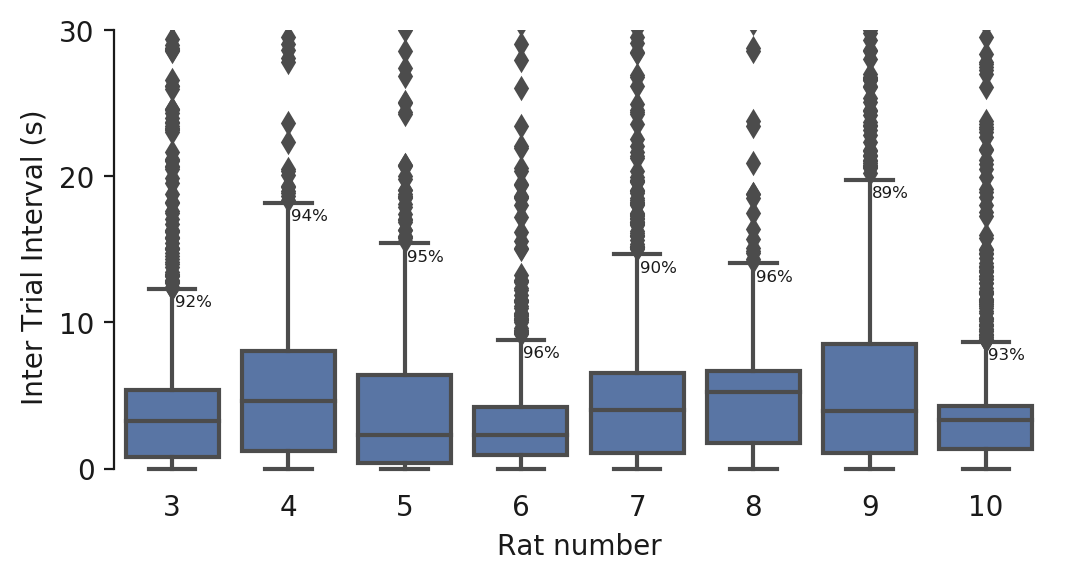
\includegraphics[width=\textwidth]{figures/inter_trial_boxplot.png}
        \caption[Time between trials is on the order of seconds]{Time between trials is on the order of seconds. The distribution of Inter Trial Intervals is shown for each rat, summarized by the boxplot quantiles. The horizontal line distanced above each box shows the last point up to 1.5 IQRs (Inter Quartile Ranges) of the .75 quartile, a common threshold to define outliers. The percentage right below that line shows how many of the points are below the threshold.}
        \label{fig:iti_box}
    \end{figure}
    
    To inquire about the animals' desire to receive rewards, we look at the period between trials, after animals have exited the nosepoke - the \textit{Inter Trial Interval}, or ITI. If animals are engaged, seeking rewards as fast as possible, then the amount of time spent in ITIs should be small. In figure \ref{fig:iti_box} we can see that most of the intervals are below 20 seconds. Specially in rats 6 and 10, more than 90\% of ITIs were under 10 seconds. Although there is variation, intervals are in the order of low tens of seconds, and thus seem to be consistent with reward seeking. On the other hand, there are many outliers: whereas figure \ref{fig:iti_box} showed up to 30s, there are some intervals with more than 10 minutes between trials. If these large intervals were distributed all along the session, this could complicate our findings. However, if they are concentrated later in the sessions, they may be indicative of natural tiredness or satiety of a previously engaged animal.
    
    \begin{figure}[ht!]
        \centering
        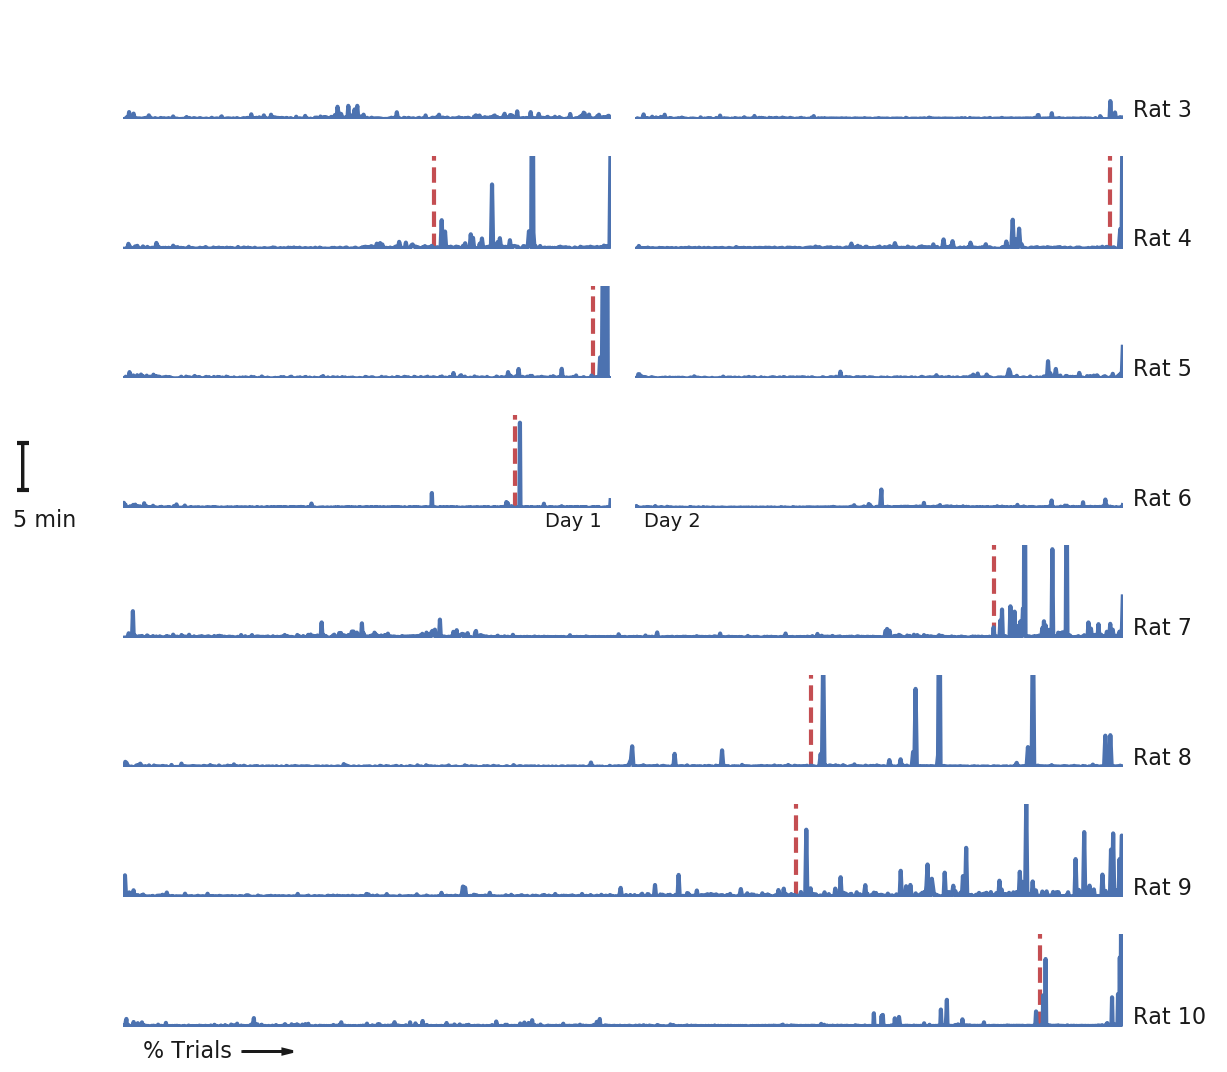
\includegraphics[width=\textwidth]{figures/inter_trial_alongtrial.png}
        \caption[Rats disengage in long sessions]{Rats disengage in long sessions, increasing their resting period between trials, waiting for minutes without engaging in the nosepoke. Each row shows the ITI of a single animal, ordered by trial, and normalized by the session duration. The upper four rows correspond to animals in the group 2, with two shorter sessions, and two respective columns. The red demarcation displays the limit of engagement, measured as the first sum of 5 or more minutes ITI in 5 consecutive trials. Posterior trials have been removed from subsequent analysis,}
        \label{fig:iti}
    \end{figure}
    
    
    To understand better how this long outlier ITIs are distributed along the session, we plotted the ITIs of each trial in sequence, in figure \ref{fig:iti}. The figure shows the two shorter sessions of animals from the group 2, and the single long session from group one. We can see that indeed the ITIs increase later in the session for almost all recorded sessions, including some of the shorter. There is some heterogeneity in the disengagement patterns: In rat 9, many medium ITIs of 1 to 5 minutes can be seen close together, with a single bigger peak. In rat 8 there are less medium ITIs, and some peaks of 10 or more minutes are separated by small ITIs (< 1 min). In rat 5, a single big peak is surrounded by small ITIs.
    
    Disregarding the heterogeneity in ITI increase, the disposition of big ITIs later in the session is consistent with the hypothesis that animals previously engaged naturally get tired (or satiated) and disengage. We wanted to define a threshold for rejecting trials after this disengagement in a reproducible manner. For such, we calculated the sum of ITIs for each 5 consecutive trials, and excluded all trials after (and including) the first sum above 5 minutes. This could be reached by a single trial with ITI bigger than 5 minutes, by five consecutive trials with 1 min of ITI each, by one ITI of 3 minutes followed by another one of 2 minutes, and so on. Figure \ref{fig:iti} shows in red the point at which sessions were pruned according to this criterion.
    
\section{Learning progression is diverse}
    \begin{figure}[ht!]
        \centering
        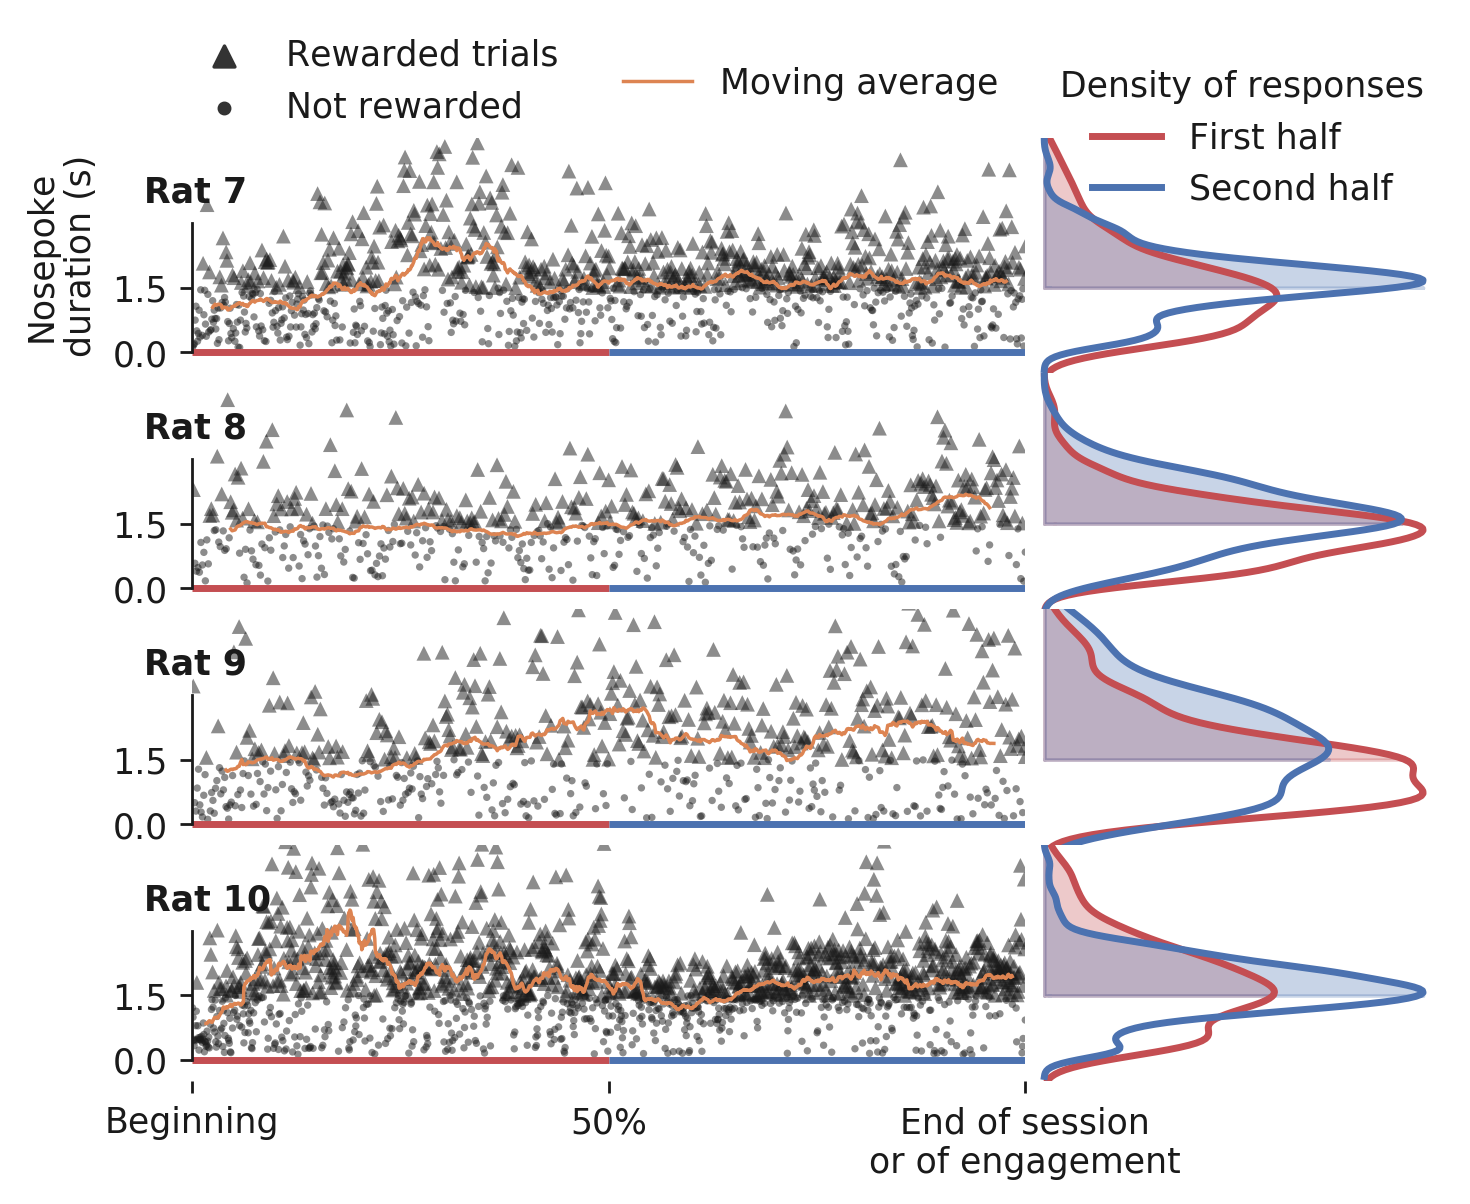
\includegraphics[width=\textwidth]{figures/behavior_group_1_with_avg_bold.png}
        \caption[Behavior across single session]{Behavior across single session, for four subjects. The circles and triangles represent the incorrect (shorter than 1.5s) and correct trials (longer than 1.5s) respectively. An orange line represents the moving average of 50 consecutive trials. The density plot on the right shows the distribution of responses in the first and second halves of the session. Rewarded trials are shaded, in such a way that the increase in rewarded trials is proportional to the difference in blue minus red shadings.}
        \label{fig:behavior}
    \end{figure} 
    
    \begin{figure}[ht!]
        \centering
        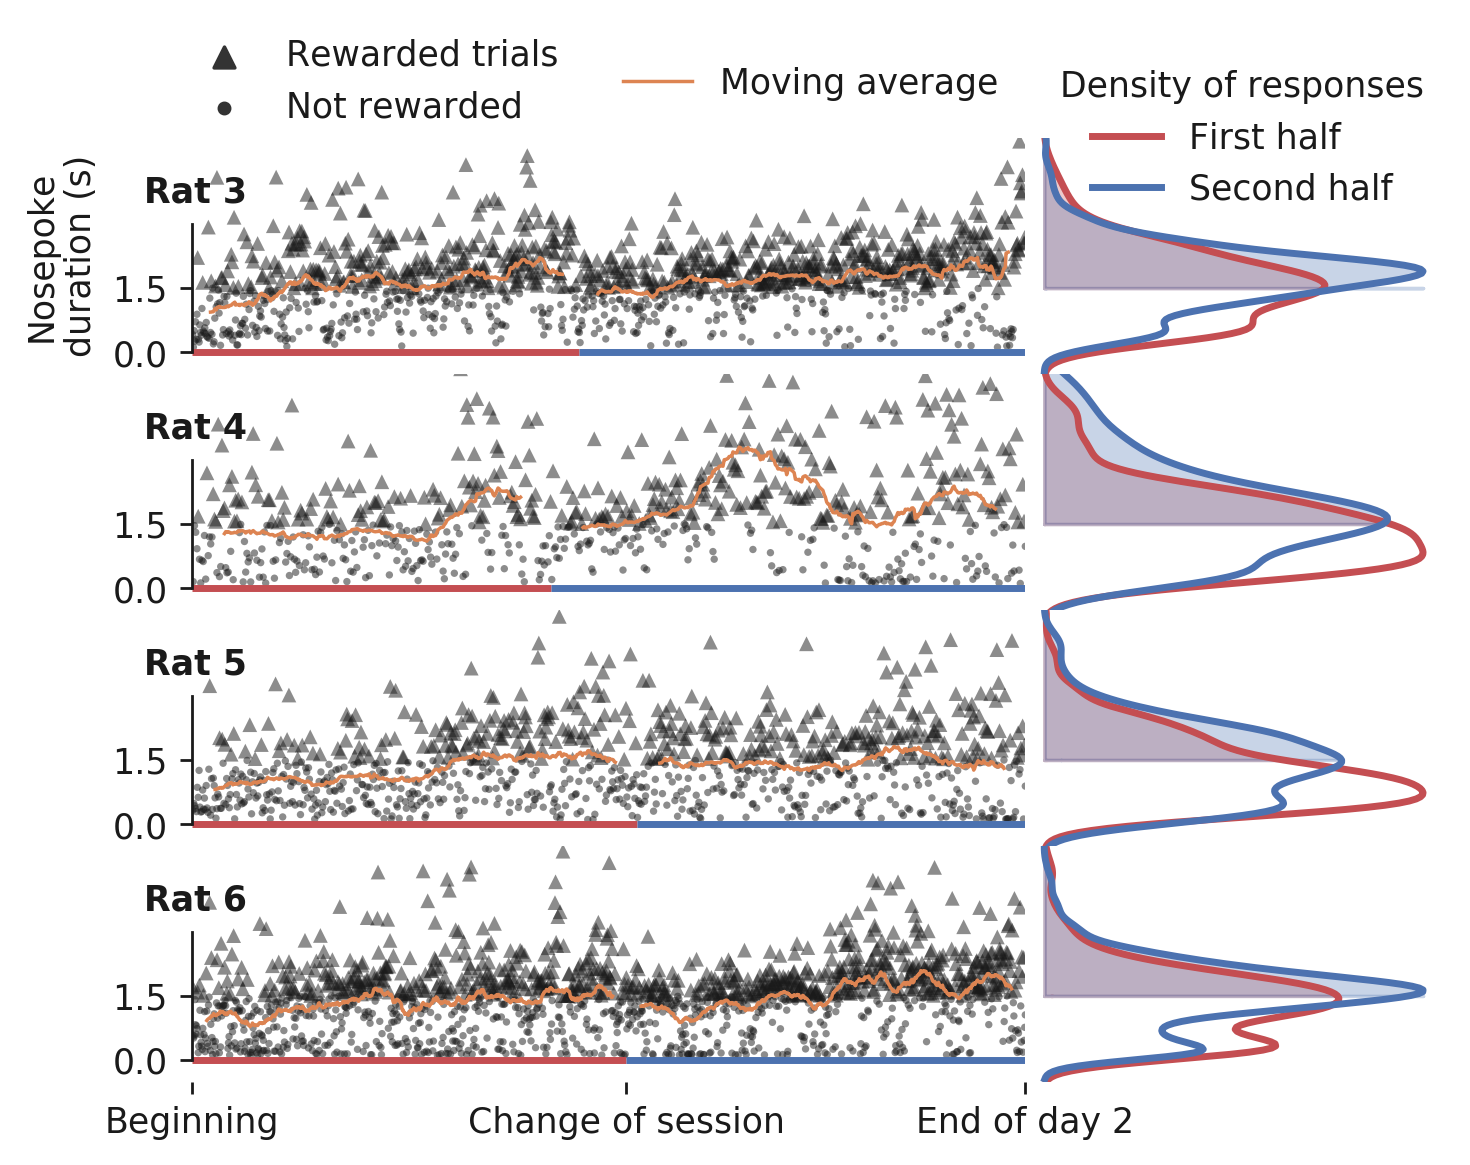
\includegraphics[width=\textwidth]{figures/behavior_group_2_with_avg_bold.png}
        \caption[Behavior across two sessions]{Behavior across two shorter sessions, for four subjects. The circles and triangles represent the incorrect (shorter than 1.5s) and correct trials (longer than 1.5s) respectively. An orange line represents the moving average of 50 consecutive trials. The density plot on the right shows the distribution of responses in the first and second sessions. Rewarded trials are shaded, in such a way that the increase in rewarded trials is proportional to the difference in blue minus red shadings.}
        \label{fig:behavior2}
    \end{figure}
    
    We show the responses for each group of animals in figures \ref{fig:behavior} and \ref{fig:behavior2}. The responses are highly variable, from milliseconds to seconds, in such a way that there are rewarded trials even early in the beginning of the session. In some animals the variability in response duration decreases perceptively (e.g. 7 and 10) and in one of them it increases (i.e. 9). This can be best seen in the density plots, showing distribution of responses in the first and second half.
    
    The moving average drifts up and down, in some rats more than in others. There are rats in which the drift is closer to monotonic. In them, variation between near trials seems smaller, for example rats 6, 8 and 9. Specially in rat 8, the moving average changes smoothly, contrasting with rats 4, 7, and 10, whose moving average has peaks early on and descends afterwards. Rat 10 reaches a moving average duration double the criterion in the first half of the session, with huge variance in its responses, before reducing the duration and variance, and centering responses around the criterion of 1.5 seconds.

\section{Rewarded responses show learning in few hundred trials}

    Looking at figures \ref{fig:behavior} and \ref{fig:behavior2}, we can see that the proportion of rewarded trials increases with training. The proportion is just the count of rewarded trials over the total number of trials. Rewarded trials are those with duration bigger than the criterion of 1.5s, and can be seen in the upper part of each behavior plot. The upper part of the density plots, above the dashed line, indicates this proportion in the area under each curve. We tested the significance of this increase separately for each group using paired-sample t-tests, and found that both are significant. This was calculated as follows: For group 1, we compared the ratio of reinforced trials in the first versus second half of the session, evaluating to p = 0.037 (T=3.564). For group 2, the first session was compared with the second, evaluating to p = 0.0002 (T=20.756). In either case, all trials after the point of no-engagement were excluded before calculation of the ratio of reinforcement.
    
    In sum, although the precise progression of response times is different for each animal, they all increase their rate of correct responses. We compared here two distinct learning stages, showing animals indeed learn and change their behavior really fast. The same learning stages will be compared with respect to their neural activity and time representation in chapter \ref{chap:rep_changes}
    